\section{Hardware Modultest (MK, PO)}

\subsection{X10-encoder}
% Generelt om Encoderens funktion
X10-encoderen er testet vha et testprogram (Henvisning til burst.cpp). Testprogrammet sender et 120kHz signal ud i 1 ms, hver gang zero cross signalet toggler. Herunder testes de enkelte blokke i encoderen.    

\subsubsection{Zero Crossing}
% Scop billede - forklaring

\begin{figure}[htb]
  \begin{minipage}{0.45\textwidth}
    \centering
      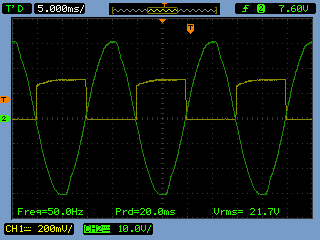
\includegraphics[width=\textwidth]{billeder/HWTest/Encoder/Encoder_zerocross}
      \caption{Zero Cross detector}
    \label{fig:ZC_UB}
  \end{minipage}
  \hspace{0.1\textwidth}
  \begin{minipage}{0.45\textwidth}
    \centering
      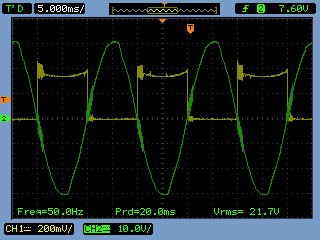
\includegraphics[width=\textwidth]{billeder/HWTest/Encoder/Encoder_zerocross_burst}
      \caption{Zero Cross detector med burst}
    \label{fig:ZC_MB}
  \end{minipage}
\end{figure}


Ud fra figur \ref{fig:ZC_UB} ses at zero Crossing detectoren virker som ønsket. Hver gang 18 Vac/50Hz passerer 0, toggles zero Cross signalet.
På figur \ref{fig:ZC_MB} ses 18Vac/50Hz signalet med burst for hver zero cross. Heraf ses at det er netop ved zero cross at 120kHz bursted placeres på 50Hz signalet. 


%\clearpage

\subsubsection{Højpasfilter}
% Scop billede - forklaring

\begin{figure}[H]
	\centering
	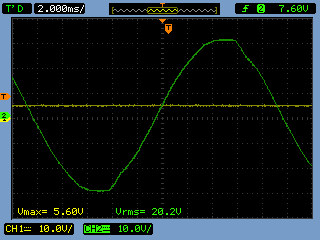
\includegraphics[width=0.50\textwidth]{billeder/HWTest/Encoder/Encoder_hojpasfilter}
	\caption{CH1:Efter højpasfilteret fra 18Vac/50Hz siden. CH2:18Vac/50Hz}
	\label{fig:HP_SCOP}
\end{figure}

Figur \ref{fig:HP_SCOP} viser begge sider af højpasfilteret. CH1 viser at 18Vac/50Hz signalet er filtreret fra. CH2 viser 18Vac/50Hz signalet fra forsyningsnettet.


\subsubsection{Output}
% Scop billede - forklaring - hvad sendes ud

\begin{figure}[htb]
  \begin{minipage}{0.45\textwidth}
    \centering
      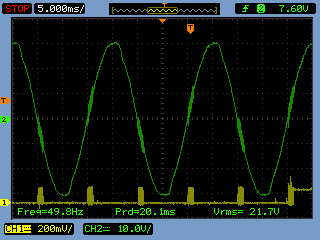
\includegraphics[width=\textwidth]{billeder/HWTest/Encoder/Encoder_50Hz_burst_120kHz}
		\caption{CH1: 120kHz burst. CH2: 18Vac/50Hz med 120kHz burst}
    \label{fig:Encoder_output}
  \end{minipage}
  \hspace{0.1\textwidth}
  \begin{minipage}{0.45\textwidth}
    \centering
      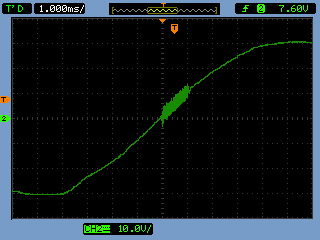
\includegraphics[width=\textwidth]{billeder/HWTest/Encoder/Encoder_burst_1ms}
		\caption{Forstørring af \ref{fig:Encoder_output}. Burst på 1ms på 18Vac/50Hz}
    \label{fig:Encoder_burst_1ms}
  \end{minipage}
\end{figure}

Herover ses figur \ref{fig:Encoder_output}. CH1 viser 120kHz burstet som sendes ud på det eksisterende forsyningsnet. CH2 viser 18Vac med 120kHz burstet fra encoderen. Det er nu decoderens opgave at afkode dette vha. X10-protokollen.

Til højre for, ses figur \ref{fig:Encoder_burst_1ms}. Dette oscilloscop billede viser at bursted er på præcis 1ms. 


\section{X10-decoder}
% Generelt om Decoderens funktion 
X10-decoderen er testet uden STK500-kittet. Det vil sige der er testet uden software på modtager delen. Testprogrammet på hovedenheden er det samme som modultesten for X10-encoderen. Et burst på 120kHz sendes ud for hvert zero cross. 

\subsection{Zero Crossing}
% Scop billede - forklaring

\begin{figure}[H]
	\centering
	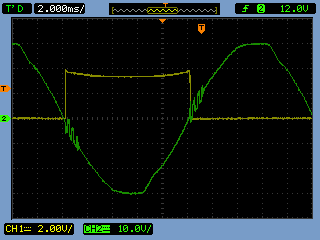
\includegraphics[width=0.50\textwidth]{billeder/HWTest/Decoder/Decoder_zerocross}
	\caption{CH1: Zero crossing firkantsignal. CH2: 18Vac/50Hz med burst for hver zero cross}
	\label{fig:Decoder_ZC}
\end{figure}

Herover ses figur \ref{fig:Decoder_ZC}. CH1 viser zero crossing detektorens firkantsignal der genereres af operationsforstærkeren når 18Vac/50Hz er negativ laver operationsforstærkeren en positiv firkant puls. CH2 viser 18Vac/50Hz signalet med 120kHz burst for hvert zero cross.   

\subsection{Båndpasfilter}
% Scop billede - forklaring

\begin{figure}[htb]
  \begin{minipage}{0.45\textwidth}
    \centering
	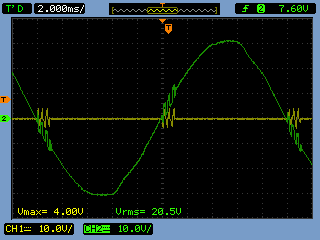
\includegraphics[width=\textwidth]{billeder/HWTest/Decoder/Decoder_hojpasfilter}
		\caption{Højpasfilterdelen af bandpasfilteret}
	\label{fig:Decoder_HP}
  \end{minipage}
  \hspace{0.1\textwidth}
  \begin{minipage}{0.45\textwidth}
    \centering
	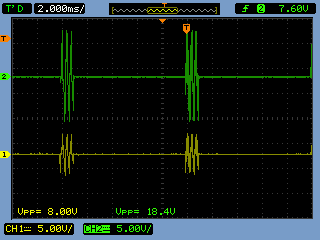
\includegraphics[width=\textwidth]{billeder/HWTest/Decoder/Decoder_forstaerkning_baandpas}
		\caption{Forstærkningen i bandpasfilteret}
	\label{fig:Decoder_Gain}
  \end{minipage}
\end{figure}

Båndpasfilteret består af et højpasfilter, en operationsforstærker samt et lavpasfilter. 
Oscilloscope billede på figur \ref{fig:Decoder_HP} viser på CH1 viser højpasfilterets funktion. Højpasfilteret filtrerer de 18Vac/50Hz fra og lader kun 120kHz signalet passere. CH2 viser inputtet fra forsyningsnettet 18Vac/50Hz med 120kHZ burst ved hvert zero cross.

Figur \ref{fig:Decoder_Gain} viser forstærkningen i båndpasfilteret. Teoretisk\footnote{Se beregninger under Båndpasfilteret \ref{Båndpasfilter}} skal der være dobbelt forstærkning. I praksis ses der at signalet (CH1) forstærkes fra 8V til 18,4V (CH2) vha. den inverterende operationsforstærker.

Det efterfølgende lavpasfilter vil igen formindste signalet. Dette ses i figur \ref{fig:Decoder_diode} på CH1 


\subsection{Envelope detector}
% Scop billede - forklaring

\begin{figure}[htb]
  \begin{minipage}{0.45\textwidth}
    \centering
	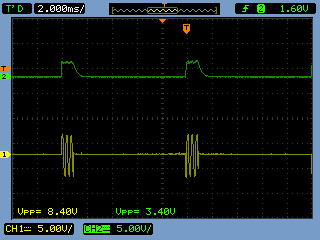
\includegraphics[width=\textwidth]{billeder/HWTest/Decoder/Decoder_ensretning}
		\caption{Ensretning dioden}
	\label{fig:Decoder_diode}
  \end{minipage}
  \hspace{0.1\textwidth}
  \begin{minipage}{0.45\textwidth}
    \centering
	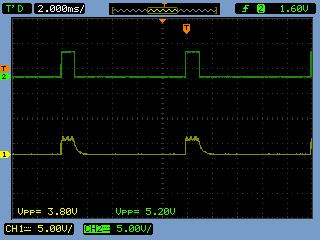
\includegraphics[width=\textwidth]{billeder/HWTest/Decoder/Decoder_envelope}
		\caption{Envelope}
	\label{fig:Decoder_envelope}
  \end{minipage}
\end{figure}

Diodens opgave er at ensrette signalet. Figur \ref{fig:Decoder_diode} viser signalet før (CH1) og efter (CH2) dioden. Toppene af 120kHz signalet samles herved og giver første billede af den ønskede firkant puls. Denne firkant puls har et max på 3,4V. Figur \ref{fig:Decoder_envelope} viser hvordan dette signal, signalet efter dioden (CH1), bliver rettet til et pænt firkantet TTL signal, som STK-500 kittet kan arbejde med, igennem envelope kredsløbet. 
  

\subsection{Output}
% Scop billede - forklaring - hvad sendes ud 
% Relæ, det aktiverer/deaktiverer udgangen via STK-500 signal 

\begin{figure}[htb]
  \begin{minipage}{0.45\textwidth}
    \centering
	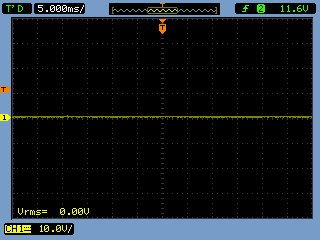
\includegraphics[width=\textwidth]{billeder/HWTest/Decoder/Decoder_relay_open}
		\caption{Deaktivt udtag}
	\label{fig:relay_open}
  \end{minipage}
  \hspace{0.1\textwidth}
  \begin{minipage}{0.45\textwidth}
    \centering
	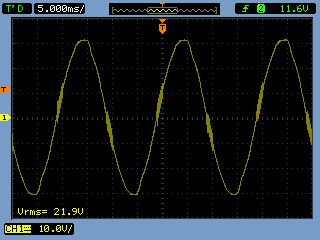
\includegraphics[width=\textwidth]{billeder/HWTest/Decoder/Decoder_relay_closed}
		\caption{Aktivt udtag}
	\label{fig:relay_closed}
  \end{minipage}
\end{figure}

Outputtet af modtageren er et 18Vac/50Hz udtag. Dette udtag er enten aktiveret eller deaktiveret. Hvis udtaget ønskes aktivt skal softwaren fungerer således at PD7 på modtager STK500 kittet sættes høj, herved aktiveres relæet og der skabes gennemgang for de 18Vac/50Hz fra forsyningsnettet. Figurene herover \ref{fig:relay_open} og \ref{fig:relay_closed} viser at udtaget enten er aktiveret eller deaktiveret. Denne test er udført ved at aktivere relæet blot fra 5V forsyningen.

\section{DE2-kodelås}

DE2 1 ms bit målt med oscilloscope på DE2 GPIO1\_D9 ift. stel. Med funktionen Trigger Single Sweep. Målingerne viser et 1 ms signal på 3.3Vpp, som ønsket.

\begin{figure}[H]
	\centering
	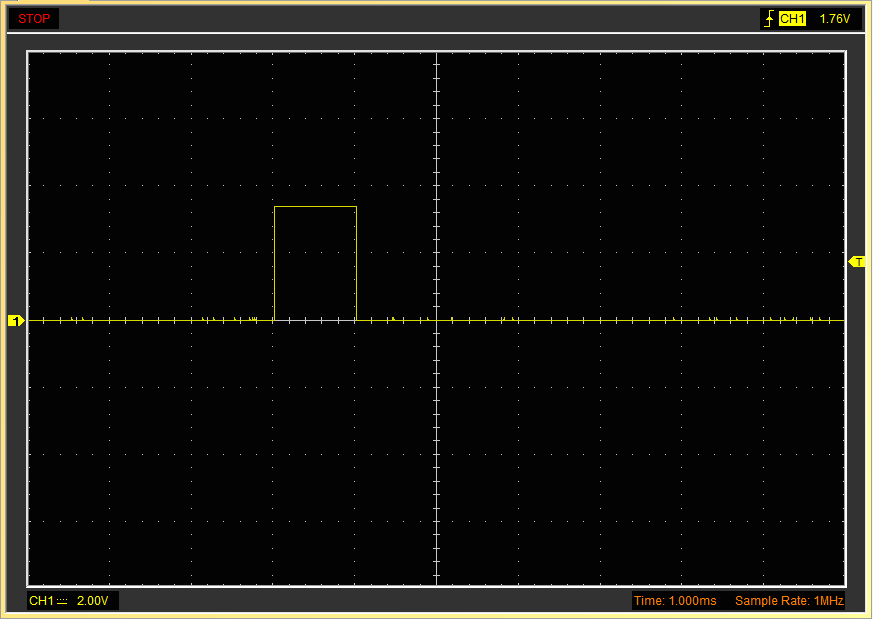
\includegraphics[width=0.50\textwidth]{billeder/HWTest/DE2/DE2_1ms_pulse}
	\caption{1 ms bit fra DE2-kodelås}
	\label{code:de2_test}
\end{figure}

\clearpage